\section{\faWrench\ Chat Memory\\{\small Concetti avanzati}} % (fold)
\label{sec:spring-ai-advanced-chat-memory}
%
\begin{frame}[t,fragile] \frametitle{Concetti avanzati}
    \framesubtitle{Per-User Chat Memory}
    {\footnotesize
    \begin{itemize}[leftmargin=10pt,align=right]
        \onslide<1->\item[\alert{\faArrowCircleRight}] Come tenere traccia di diverse conversazioni?
        \begin{itemize}[leftmargin=10pt,align=right]
            \onslide<2->\item[\alert{\faArrowCircleRight}] \texttt{ChatMemory} definita secondo una logica \alert{multi-conversazione}
            \onslide<3->\begin{itemize}[leftmargin=10pt,align=right]
                \item[\alert{\faExclamationTriangle}] \alert{\texttt{CONVERSATION\_ID}} chiave che il sistema ricerca nel contesto per CRUD storico messaggistica
                \item[\alert{\faExclamationTriangle}] \alert{\texttt{DEFAULT\_CONVERSATION\_ID}} valore di \textit{default} fornito alla chiave se non popolata programmaticamente
            \end{itemize}
        \end{itemize}
    \end{itemize}
    }
    \begin{block}{Interfaccia Chat Memory}
		{\tiny\inputminted{java}{code/ChatMemory.java}}
    \end{block}
\end{frame}    
%
\begin{frame}[t,fragile] \frametitle{Concetti avanzati}
    \framesubtitle{Per-User Chat Memory}
    \vspace*{-.7cm}
    {\footnotesize
    \begin{itemize}[leftmargin=10pt,align=right]
        \onslide<1->\item[\alert{\faArrowCircleRight}] Come sovrascrivere il valore di \textit{default}?
        \begin{itemize}[leftmargin=10pt,align=right]
            \onslide<2->\item[\alert{\faArrowCircleRight}] Agire a livello di \textit{chat memory advisor}
            \onslide<3->\item[\alert{\faArrowCircleRight}] Utilizzo delle \textit{advisor specifications} di \texttt{ChatClient} (\alert{\texttt{ChatClient\$AdvisorSpec}})
        \end{itemize}
    \end{itemize}
    \onslide<2->
    \begin{block}{Interfaccia per ogni \textit{chat memory advisor}}
		{\tiny\inputminted{java}{code/BaseChatMemoryAdvisor.java}}
    \end{block}
    \onslide<3->
    \begin{block}{Customizzazione \textit{id} conversazione}
		{\tiny\inputminted{java}{code/AdvisorSpecExample.java}}
    \end{block}
    }
\end{frame}
%
\begin{frame}[t,fragile] \frametitle{Progetto Spring AI}
    \framesubtitle{Applicazione e passaggi}
    {\small
    \begin{itemize}[leftmargin=10pt,align=right]
        \item[\alert{\faArrowCircleRight}] Configurazione \textit{per-user chat memory} per \texttt{ChatClient} Ollama
        \begin{itemize}[leftmargin=10pt,align=right]
            \onslide<2->\item[\alertedcircled{1}] Creazione modello per richiesta domanda con \textit{username}
            \onslide<3->\item[\alertedcircled{2}] Modifica interfaccia e implementazione del servizio di risposta
            \onslide<4->\item[\alertedcircled{3}] Modifica controllore MVC
            \onslide<5->\item[\alertedcircled{4}] \textit{Test} delle funzionalità con Postman/Insomnia
        \end{itemize}
    \end{itemize}
    }
\end{frame}
%
\begin{frame}[t,fragile] \frametitle{Progetto Spring AI}
    \framesubtitle{Per-user chat memory}
        \begin{block}{Modello richiesta con \textit{username}}
			{\tiny\inputminted{java}{code/QuestionRequest.java}}
    	\end{block}
\end{frame}
%
\begin{frame}[t,fragile] \frametitle{Progetto Spring AI}
    \framesubtitle{Per-user chat memory}
        \begin{block}{Interfaccia servizio}
			{\tiny\inputminted{java}{code/QuestionService.java}}
    	\end{block}
\end{frame}
%
\begin{frame}[t,fragile] \frametitle{Progetto Spring AI}
    \framesubtitle{Per-user chat memory}
        \vspace*{-.7cm}
        \begin{block}{Implementazione servizio}
			{\tiny\inputminted{java}{code/QuestionServiceImpl.java}}
    	\end{block}
\end{frame}
%
\begin{frame}[t,fragile] \frametitle{Progetto Spring AI}
    \framesubtitle{Per-user chat memory}
    	\vspace*{-.7cm}
        \begin{block}{Implementazione controllore REST}
			{\tiny\inputminted{java}{code/QuestionController.java}}
    	\end{block}
\end{frame}
%
\begin{frame}[fragile] \frametitle{Codice}
    \framesubtitle{Branch di riferimento}
	\begin{center}
		{\scriptsize \href{https://github.com/simonescannapieco/spring-ai-advanced-dgroove-venis-code.git}{\texttt{https://github.com/simonescannapieco/spring-ai-advanced-dgroove-venis-code.git}}}\\
		\textit{Branch:} \alert{\texttt{5-spring-ai-gemini-ollama-per-user-chat-memory}}
	\end{center}
\end{frame}
%
\begin{frame}[t,fragile] \frametitle{Concetti avanzati}
    \framesubtitle{Persistent Chat Memory}
    {\footnotesize
    \begin{itemize}[leftmargin=10pt,align=right]
        \onslide<1->\item[\alert{\faExclamationTriangle}] Storico della conversazione valida per singola sessione
        \begin{itemize}[leftmargin=10pt,align=right]
            \onslide<2->\item[\alert{\faArrowCircleRight}] Opzione valida per demo/applicazioni a bassa criticità
            \onslide<3->\item[\alert{\faArrowCircleRight}] Possibile \alert{persistere} le informazioni di storico su DB
            \begin{itemize}[leftmargin=10pt,align=right]
                \item[\alert{\faArrowCircleRight}] PostgreSQL
                \item[\alert{\faArrowCircleRight}] MySQL/MariaDB
                \item[\alert{\faArrowCircleRight}] SQL Server
                \item[\alert{\faArrowCircleRight}] HSQLDB
            \end{itemize}
        \end{itemize}
        \begin{block}{Dipendenza di progetto}
			{\tiny\inputminted{xml}{code/pom.xml}}
    	\end{block}
    \end{itemize}
    }
\end{frame}
%
\begin{frame}[t,fragile] \frametitle{Concetti avanzati}
    \framesubtitle{Persistent Chat Memory - Esempio minimale}
    \vspace*{-.7cm}
    \begin{block}{Definizione \textit{bean}}
		{\tiny\inputminted{java}{code/jdbcChatMemoryExample.java}}
    \end{block}
    \onslide<2->
    \begin{itemize}[leftmargin=10pt,align=right]
        \item[\alertedcircled{1}] Il sistema inferisce la tipologia di DB dalle proprietà dell'applicativo
    \end{itemize}
    \begin{block}{File \texttt{application.yml}}
		{\tiny\inputminted{yaml}{code/application.yml}}
    \end{block}
    \onslide<3->
    \begin{itemize}[leftmargin=10pt,align=right]
        \item[\alertedcircled{2}] Il sistema applica lo schema relativo al DB inferito
    \end{itemize}
    \begin{block}{File \texttt{schema-postgresql.sql}}
		{\tiny\inputminted{sql}{code/schema-postgresql.sql}}
    \end{block}
\end{frame}
%
\begin{frame}[t,fragile] \frametitle{Concetti avanzati}
    \framesubtitle{Definizione nuovo connettore}
    \vspace*{-.7cm}
    {\small
    \begin{itemize}[leftmargin=10pt,align=right]
        \only<1|handout:1>{\item[\alertedcircled{1}] Definire un nuovo schema per il nuovo connettore}
        \only<2|handout:2>{\item[\alertedcircled{2}] Impostare i corretti parametri dell'applicativo}
    \end{itemize}
    \only<1|handout:1>{
    \begin{block}{File \texttt{./resources/schema/schema-h2.sql}}
		{\tiny\inputminted{sql}{code/schema-h2.sql}}
    \end{block}}
    \only<2|handout:2>{
    \begin{block}{File \texttt{application.yml}}
		{\tiny\inputminted{yaml}{code/application-2.yml}}
    \end{block}
    \begin{block}{File \texttt{pom.xml}}
		{\tiny\inputminted{xml}{code/pom-2.xml}}
    \end{block}
    }
    }
\end{frame}
%
\begin{frame}[t,fragile] \frametitle{Progetto Spring AI}
    \framesubtitle{Applicazione e passaggi}
    {\small
    \begin{itemize}[leftmargin=10pt,align=right]
        \item[\alert{\faArrowCircleRight}] Configurazione \textit{JDBC H2 chat memory} per \texttt{ChatClient} Ollama
        \begin{itemize}[leftmargin=10pt,align=right]
            \onslide<2->\item[\alertedcircled{1}] Modifica al \texttt{pom.xml} per dipendenze Spring AI JDBC, H2 e \textit{devtools}
            \onslide<3->\item[\alertedcircled{2}] Modifica ad \texttt{application.yml}
            \onslide<4->\item[\alertedcircled{3}] Creazione schema H2
            \onslide<5->\item[\alertedcircled{4}] Modifica ai \textit{bean} \texttt{ChatClient} per Ollama
            \onslide<6->\item[\alertedcircled{5}] \textit{Test} delle funzionalità con Postman/Insomnia
        \end{itemize}
    \end{itemize}
    }
\end{frame}
%
\begin{frame}[t,fragile] \frametitle{Progetto Spring AI}
    \framesubtitle{JDBC chat memory}
        \begin{block}{Dipendenze di sistema aggiuntive}
			{\tiny\inputminted{xml}{code/pom-3.xml}}
    	\end{block}
\end{frame}
%
\begin{frame}[t,fragile] \frametitle{Progetto Spring AI}
    \framesubtitle{JDBC chat memory}
        \begin{block}{Configurazione applicativo}
			{\tiny\inputminted{yaml}{code/application-2.yml}}
    	\end{block}
\end{frame}
%
\begin{frame}[t,fragile] \frametitle{Progetto Spring AI}
    \framesubtitle{JDBC chat memory}
        \begin{block}{Schema H2}
			{\tiny\inputminted{sql}{code/schema-h2.sql}}
    	\end{block}
\end{frame}
%
\begin{frame}[t,fragile] \frametitle{Progetto Spring AI}
    \framesubtitle{JDBC chat memory}
    	\vspace*{-.7cm}
        \begin{block}{Configurazione Gemini + Ollama}
			{\tiny\inputminted{java}{code/MemoryChatClientConfig.java}}
    	\end{block}
\end{frame}
%
\begin{frame}[t,fragile] \frametitle{Ambiente di sviluppo}
\framesubtitle{Popolamento Vector Store}
	\vspace*{-.5cm}
    {\footnotesize
    \begin{itemize}
        \item[\alert{\faExclamationTriangle}] Verificare la \textit{dashboard} H2 (\texttt{http://localhost:8080/h2-console})
    \end{itemize}
    }
    \vfill
    \begin{minipage}[b]{\textwidth}
		\centering
		    \begin{figure}[ht]
			    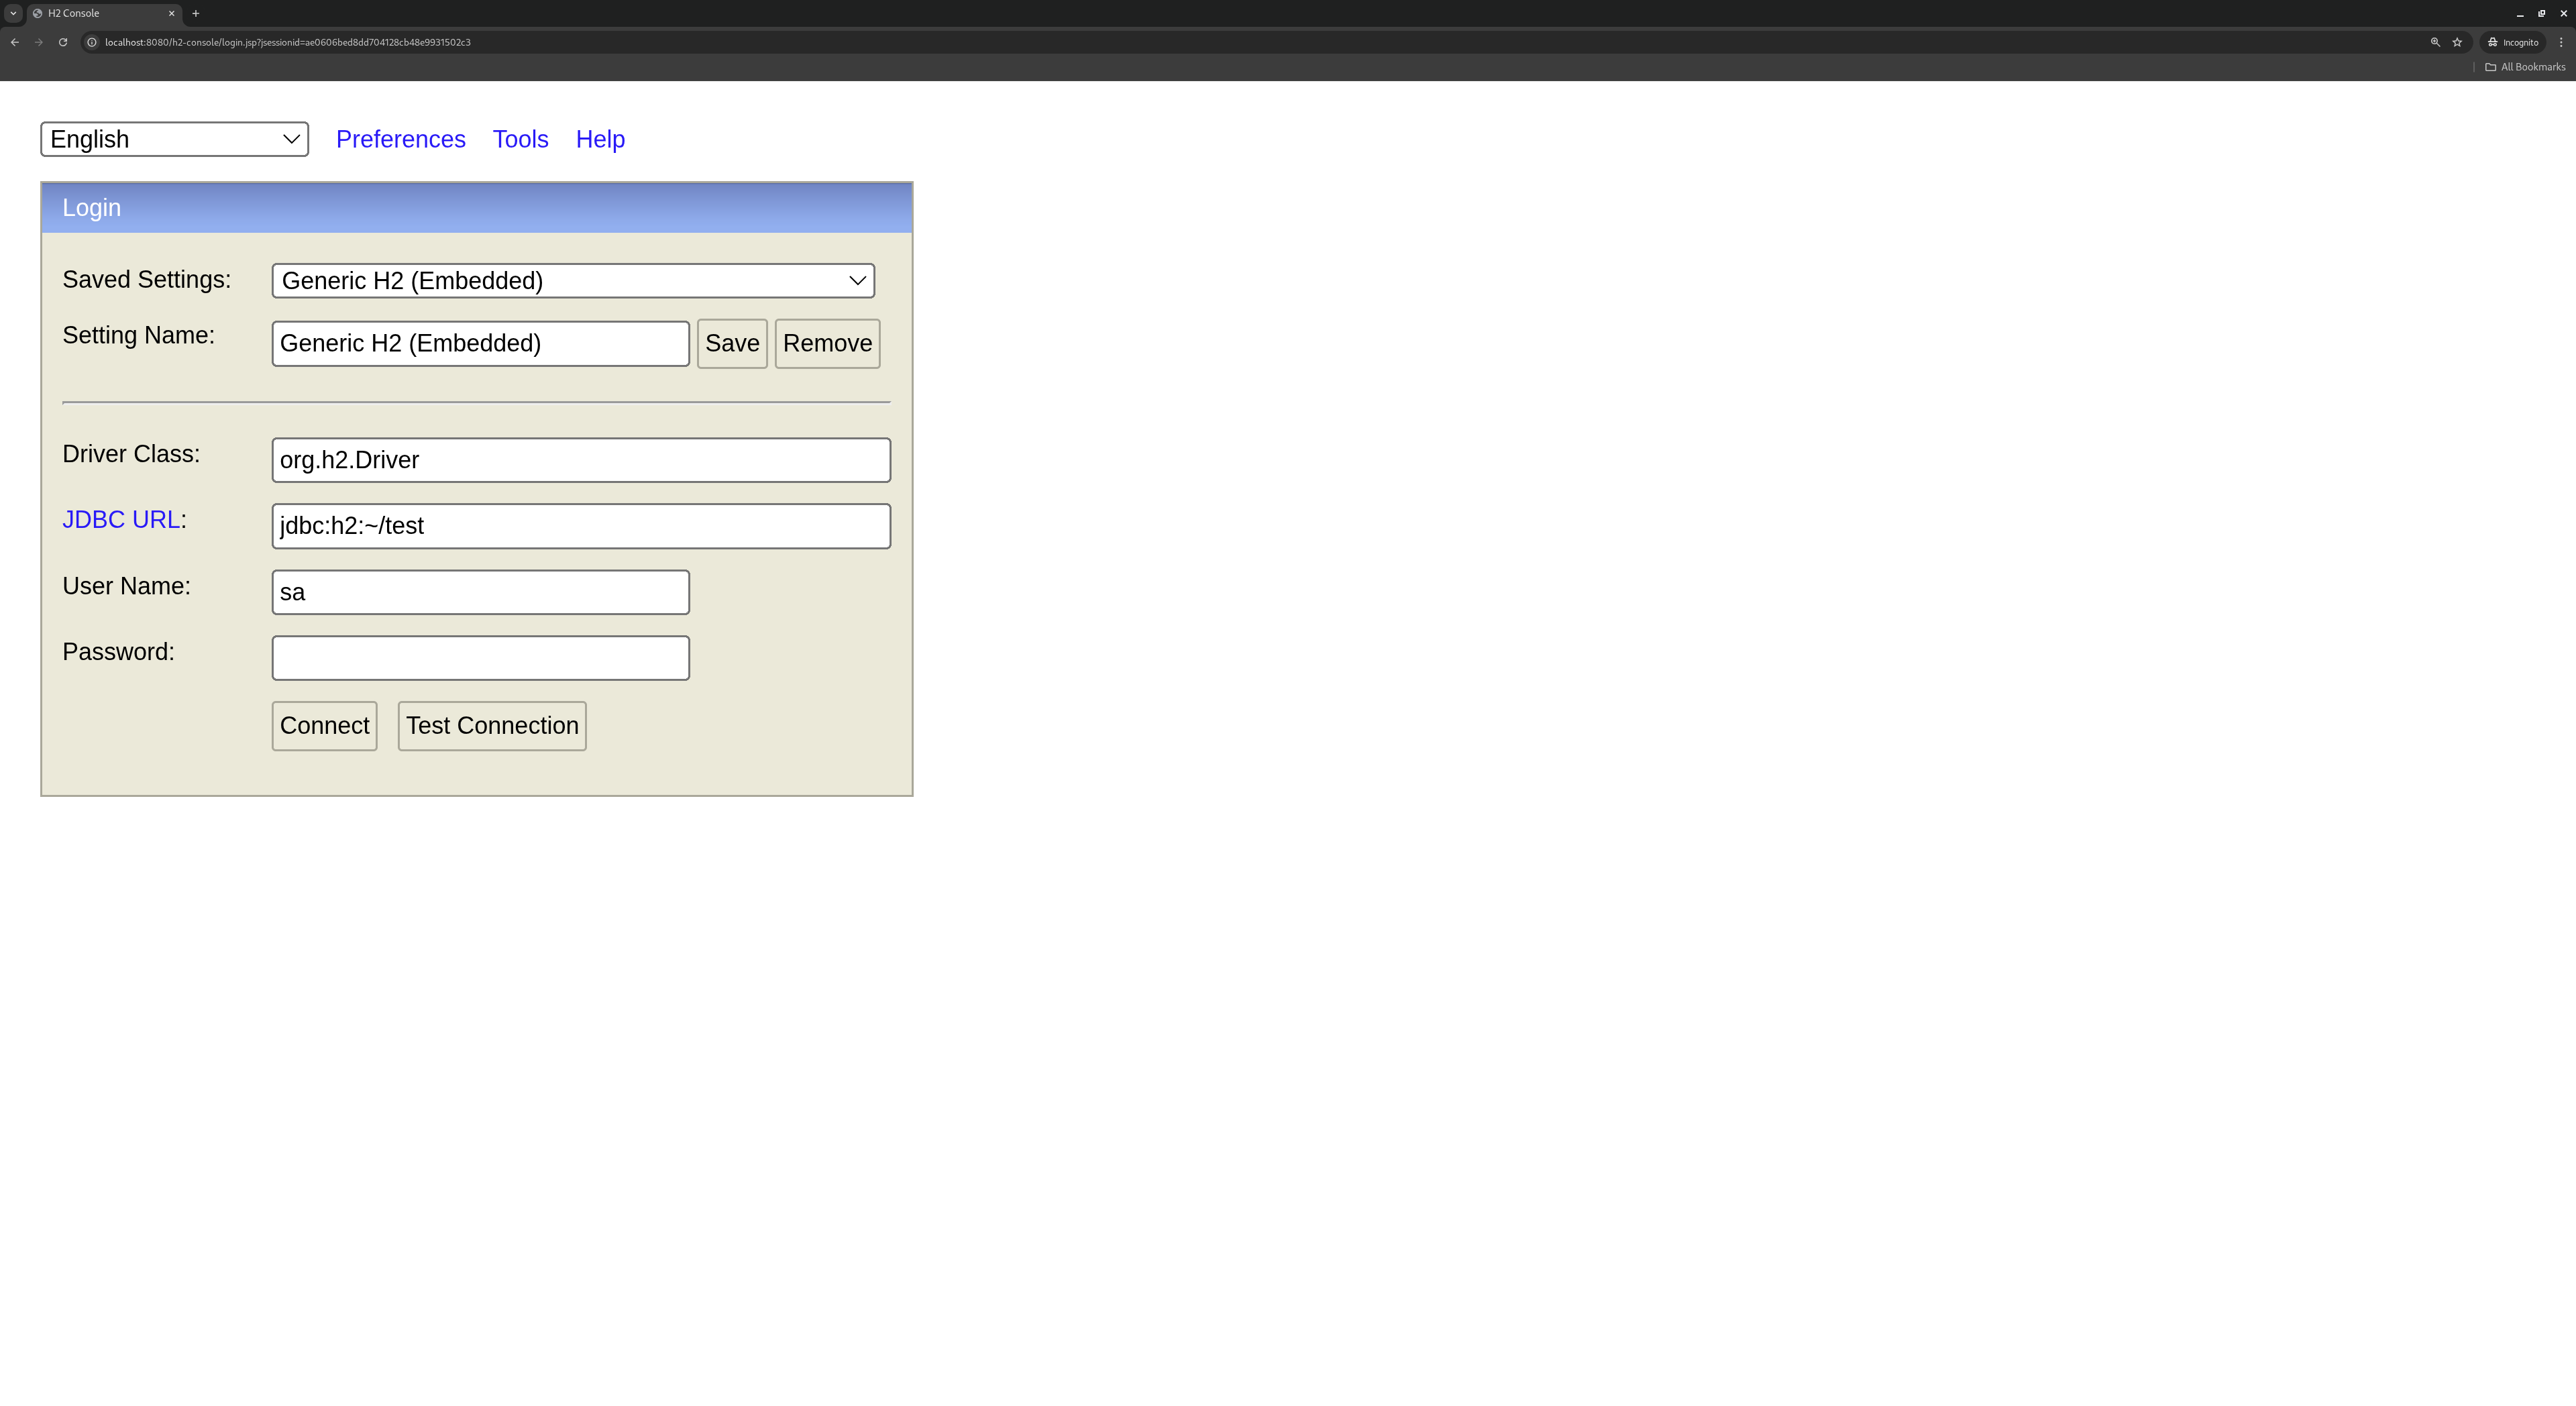
\includegraphics[width=\textwidth, frame]{img/h2-console.png}
		    \end{figure}
	\end{minipage}
\end{frame}
%
\begin{frame}[fragile] \frametitle{Codice}
    \framesubtitle{Branch di riferimento}
	\begin{center}
		{\scriptsize \href{https://github.com/simonescannapieco/spring-ai-advanced-dgroove-venis-code.git}{\texttt{https://github.com/simonescannapieco/spring-ai-advanced-dgroove-venis-code.git}}}\\
		\textit{Branch:} \alert{\texttt{6-spring-ai-gemini-ollama-jdbc-chat-memory}}
	\end{center}
\end{frame}